% #############################################################################
% This is Chapter 5
% !TEX root = ../main.tex
% #############################################################################
% Change the Name of the Chapter i the following line
\fancychapter{Exploring parameters-efficient transfer learning for end-to-end children ASR}
\label{chap:Adapters_exp}
\cleardoublepage

\section{Introduction}
The use of increasingly larger models coupled with the abundance of massive datasets is driving rapid advancements in many domains of machine learning, encompassing NLP \cite{brown2020language} and computer vision \cite{ramesh2021zero}. In the context of ASR, this trend of scalling up models is exemplified by state-of-the-art models such as Whisper \cite{radford2023robust} and HuBert \cite{hsu2021hubert}, where the number of parameters exceeds 1 billion. Research has underscored the interconnected nature of the training dataset size and the number of model parameters, identifying them as mutual bottlenecks that influence the performances of machine learning models. This observation accentuates the significance of scaling these two dimensions in tandem for the development of more robust and effective ASR models \cite{Kaplan2020ScalingLF}. Typically, to scalling up the model size a combination of an increased number of layers and an expansion of the model's hidden dimensions is used \cite{zheng22d_interspeech}.

However, the challenge arises when only a limited amount of data is available, making it challenging to train these large models from scratch, as highlighted by recent studies \cite{sri_end2end, gelin2021endtoend}. Hence, as discussed in the preceding chapter, transfer learning emerges as a well-established and effective paradigm to tackle to problematic of limited dataset. Nevertheless, despite its efficacy, we emphasised certain limitations that may potentially impede the performance of fine-tuning. Specifically, attempting to fine-tune these large models using a downstream dataset limited in size can be challenging. Indeed, in addition to be an expensive process, using small amount of data on such big model could potentially result in overfitting. This issue necessitates careful consideration, particularly in light of the recent evolution towards ever-growing pre-trained model sizes. Additionally, even following last chapter highlights where only specific parts of the model were fine-tuned, the different part of the model could be intricately linked to the overall model size. For example, FFN modules usually represent substantial portion, around 70\% of the total number of parameters. This insight underscores the persistence of the challenge associated with model size, even when fine-tuning only specific components. Finally, TL on large amount of parameters is memory-storage-inefficient, especially when there is a need to store a replicas of the billion of parameters models for many different small tasks.

Consequently, there is a growing need for more parameter-efficient transfer learning (PETL) as lightweight alternatives.
 %The use of increasingly bigger models in conjunction with the availability of massive datasets is driving rapid advancements across various domains of machine learning, including NLP and computer vision. In the context of ASR, this scaling up evolution is illustrated by state-of-the-art models such as Whisper and HuBert, where the number of parameters surpass 1 billion. Some research underscored the interconnected nature of the size of the training dataset and the number of parameters in model, as they both act as mutual bottlenecks in the pursuit of enhancing machine learning models. This critical observation highlight the importance of scaling these two dimensions in tandem for the development of better ASR models. Typically, the augmentation of the model's size results from a combination of an increased number of layers and an expansion of the model's hidden dimensions.
%However, when only limited amount of data is available it can be challenging to train these model from sratch \cite{sri_end2end,gelin2021endtoend}. Therefore, as discussed in the previous chapter, transfer learning emerges as a well-established and effective paradigm in this comtext. Nevertheless, despite its effectiveness, we underscored certain limitations that may potentially impede the efficacy of fine-tuning. Notably, challenges arise when fine-tuning large models using a downstream dataset limited in size. This is a crucial issue that requires careful consideration, particularly in light of the recent evolution of ever-growing size of pre-trained model. In addition, the process of fine-tuning specific parts of the model, such as the FFN modules for the Transformer, is intricately linked to the model size, as FFN modules often represents $\frac{2}{3}$ of the total amount of parameters.There is, then, a need for more parameters efficent approaches. Furthermore, TL from the large amount of parameters is storage-inefficient, especially when fine-tuning a model of billion of parameters for a lot of different small tasks. 
%In this context, the research community has introduced several parameter-efficient transfer learning (PETL) as a lightweight alternatives.
 Among the approaches introduced by the research community, residual Adapter modules stand out as the most popular and promising \cite{houlsby, pfeiffer}. Specifically tailored for Transformer-based systems, Adapters integrate a compact set of additional layers into a pre-trained source model. This design enables Adapters to enhance computational efficiency, resulting in faster training and addressing the challenge of catastrophic forgetting. Diverging from conventional transfer learning methods, where the source pre-trained model's weights are entirely replaced, Adapter-transfer maintains the integrity of the backbone model. Therefore, when the Adapter modules are removed, the initial pre-trained model remains unchanged. This preservation of the backbone model is a crucial advantage  as it offer increased flexibility. Furthermore, owing to their limited number of trainable parameters, Adapters demonstrate a decreased susceptibility to overfitting, thereby contributing to improved generalisation performance.


 In this chapter, motivated by these promising characteristics, our investigation will delve into the use of Adapters in the specific context of children's ASR. We will explore different Adapter configurations within both Transformer and Conformer architectures. Additionally, as a comparative analysis to Adapters, we will explore the application of other PETL approaches in the context of children's ASR. Lastly, we will introduce a novel type of Adapter, referred to as shared-Adapters, taking advantage from the overparameterisation inherent in Transformer-based models.


%In this context, the research community has introduced several parameter-efficient transfer learning (PETL) as a lightweight alternative.  Among these differents approaches, residual Adapter modules represents the most popular and promising PETL. Specifically designed for Transformer-based systems, Adapters integrate a compact set of additional layers into a pre-trained source model \cite{houlsby, pfeiffer}. This design allows Adapters to enhance computational efficiency, facilitating faster training and mitigating the issue of catastrophic forgetting.

%In contrast to conventional transfer learning approaches, where the source model's weights are entirely replaced, adapter transfer preserves the backbone model. Even when the adapter layers are removed, the underlying model remains unchanged. This retention of the backbone model provides a valuable advantage, allowing for greater flexibility and adaptability. Moreover, due to their limited number of trainable parameters, adapters exhibit a reduced susceptibility to overfitting, contributing to improved generalisation performances. Motivated by this, we will investigate ther use of ADapter in the context of children's ASR in this chapter. Different configuration in the context of both Transfromer and Conformer will be presented. Then, as comparaison to Adapter we will investigate the use of other PETL in the context of children ASR. Finally, we will propose a new type of Adapter, the shared-Adapters, that use the overparameterisation present in Transformer-based model to reduce the number of parameters.



%In response to these challenges, the research community has introduced lightweight alternatives for fine-tuning, known as parameter-efficient transfer learning (PETL).Residual adapter modules represents an popular PETL approach, especially to address the problems in traditional transfer learning. Adapters, specifically designed for Transformer-based systems integrate a compact set of additional layers into a pre-trained source model \cite{houlsby, pfeiffer}. These Adapters typically provide enhanced computational efficiency, resulting in faster training and mitigating the problem of catastrophic forgetting. In contrast to conventional transfer learning, where the source model's weights are completely replaced, adapter transfer preserves the backbone model, leaving it unchanged even when the adapter layers are removed. Additionally, due to their limited number of trainable parameters, adapters tend to be less prone to over-fitting.
%As presented in the previous chapter, transfer learning, despite beeing a well-established and well-performing paradigm has some limitations. Especially when it comes to fine-tuning large models with a limited-size downstream dataset. However, the availability of massive datasets and the development of ever-growing size model allowed rapid progress in many field of machine learning, from NLP, computer vision and ASR. Examples of such models like Whisper and HuBert can go up to more than 1 billion parameters. In addition, the size of the training dataset and the number of model parameters are mutual bottlenecks and must be scaled in tandem, which is a important information for the development of better ASR models.  Usually, the models size are increase by a conjounction of increased number of layer, model's dimension.  As a consequence, fine-tuning part of the model, such as the FFN layers only, can also drasticly increase. 
%More recently, advances on self-supervised learning (SSL)  focused on training models to extract representations from large volumes of unsupervised data. Subsequently, the entire network undergoes fine-tuning to use the extracted representations effectively in supervised tasks. Notably, these advances have led to significant improvements in child speech recognition\cite{9847929,fan2022draft}. However, fine-tuning the entire network in this way can lead to significant computational costs, including long training times and substantial storage requirements. Moreover, SSL is vulnerable to domain shift, when the data domain used for fine-tuning differs from the initial pre-training domain. Although SSL yields improved performances with extensive unlabeled data during pre-training, recent research suggests that even greater improvements can be achieved by including target domain data during the pre-training phase \cite{hwang2022large}.
%However, larger models require more data for effective fine-tuning to prevent over-fitting. 
%Residual adapter modules offer an alternative approach to address traditional transfer learning limitations in the context of automatic children's speech recognition of large ASR models. Adapters, specifically designed for Transformer-based systems integrate a compact set of additional layers into a pre-trained source model \cite{houlsby, pfeiffer}. These adapters typically provide enhanced computational efficiency, resulting in faster training and mitigating the problem of catastrophic forgetting. In contrast to conventional transfer learning, where the source model's weights are completely replaced, adapter transfer preserves the backbone model, leaving it unchanged even when the adapter layers are removed. Additionally, due to their limited number of trainable parameters, adapters tend to be less prone to over-fitting.

%In this chapter, we extend research presented in \cite{chen2023efficient} and \cite{10095837} by conducting a comprehensive evaluation of various adapter  and other PETL configurations specifically designed for Conformer models in the domain of children's speech recognition. Furthermore, we introduce a two adapter configurations, the Two Serial Adapter (TSA) and Shared-Adapter. We also considering the potential benefits of age-dependent acoustic models, and given the strong correlation between children's age and acoustic variability \cite{gale2019improving, shivakumar2020transfer}, we propose a novel cluster-based strategy for training adapters.

\section{Adapters}

\begin{figure*}[t]
    \begin{center}
    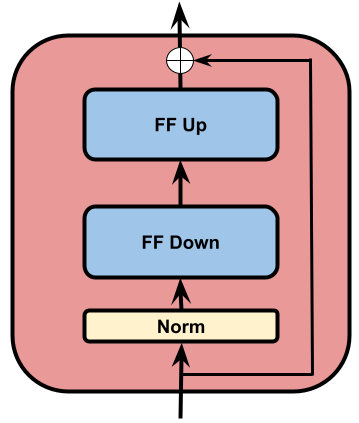
\includegraphics[scale=0.3]{imgs/Adapter_alone.png}
    \caption{Residual Adapter architecture}
    \label{fig:Adapter_architecture}
    \end{center}
    \end{figure*}


Adapters were initially introduced in the NLP field to efficiently adapt large models, such as Transformers, using minimal amount of parameters for text classification \cite{houlsby}. As an alternative to full model fine-tuning, Adapter-transfer involves training an extra small number of task-specific parameters while keeping the original model frozen. This is done at each Transformer layer level by plugging them after the Multi-Head Attention (MHA) and Feedforward Neural Network (FFN) modules, a setup often referred to as the \textit{Houlsby} configuration. Subsequently, \cite{pfeiffer} demonstrated that Adapters placed only after the FFN modules were sufficient for achieving efficient performances, referred to as the \textit{Pfeiffer} configuration. Generally, Adapters employ a bottleneck architecture, consisting of a normalisation layer followed by a projection-down linear layer with a non-linear activation, and subsequently a projection-up linear layer. Finally, a residual connection is applied by summing the input of the Adapter with its output. The overall structure is illustrated in Figure \ref{fig:Adapter_architecture}. Research suggests that the hidden dimension, between the down and up projections, may not always benefit from a bottleneck structure, where $d_{hidden} < d_{model}$, and the optimal design may vary depending on the downstream task. In some tasks, an hidden dimension larger than the model size itself, in other words $d_{hidden} > d_{model}$, has been proven more effitive \cite{fan2022draft}.

Some of the main advantages of Adapters are their parameter efficiency and modularity. This efficiency is particularly interesting when working with large pre-trained models, while the modularity is valuable when a large number of tasks need to be trained.
Mathematically, the structure of an Adapter can be expressed as follows:
%Adapters were first introduced in the natural language processing field to efficiently adapt large models like Transformers for text classification \cite{houlsby}. They are a simple alternative to full model fine-tuning, adding a small number of parameters at each transformer layer, generally after the feed-forward layer. Adapters use a bottleneck architecture (projection-down followed by projection-up) and have benefits such as parameter efficiency, faster training, and modularity compared to full fine-tuning. Adapter can be expressed as follows:
\begin{equation}
    adapter(x) = x + (W_{up}(f(W_{down}g(x)+b_{down})))+ b_{up})
\end{equation}
Where $W_{down}$ and $W_{up}$ denote the weights of the projection-down and projection-up linear layers, and $b_{down}$ and $b_{up}$ represent the corresponding biases. The function $f(\cdot)$ is a non-linear activation, while $g(\cdot)$ a layer normalisation or identity function. Finally, $x$ corresponds the input given to the Adapter.

In terms of computation, Adapters offer the advantage of faster training, given that they update fewer parameters compared to fully fine-tuning models. However, there might be a slight processing delay during inference due to the addition of extra parameters introduced by the Adapters, this difference is generally minimal and can be well-managed \cite{ruckle2020adapterdrop}.

% Adapter ASR
Adapter-transfer has gained increased attention in the context of ASR tasks \cite{cappellazzo2023parameter,chen2023efficient,10095837}, particularly owing to its modular nature, which has proven advantageous in the context of multi-lingual ASR \cite{kannan2019large, hou2021exploiting, kulkarni2023adapting}. In these studies, distinct Adapters were trained for each language, contributing to enhanced performance compared to a monolingual model and mitigating certain challenges associated with transfer learning, such as overfitting. This modular approach provides a tailored solution, as each Adapter designed for a specific language can effectively capture the diverse acoustic characteristics unique to that language.



In addition, researchers have explored the use of Adapters in the context of SSL. In SSL, larger model are typically employed to capture a wide range of information from speech for application in a broad spectrum of tasks \cite{thomas2022efficient, fan2022draft}. However, the computational cost and scalability to multiple tasks can pose a challenge. Notably, once the model is fine-tuned for a specific task, the entire model is fixed for that task, and re-loading and re-training the base model are necessary for transferring to a different task. Therefore, the use of Adapters has proven effective in addressing these challenges by providing a modular and parameter-efficient task-specific adaptation.


Additionally, the effectiveness of Adapters has been demonstrated in addressing challenges related to low-resource and atypical speech recognition scenarios \cite{tomanek2021residual}

Finally, the effectiveness of Adapters has also been demonstrated in addressing challenges related to low-resource and atypical speech recognition scenarios \cite{tomanek2021residual}. In such scenarios, similarly to children's speech, there is limited availability of labeled data and atypical speech characteristics. As a result, Adapters provide a valuable solution by efficiently adapting large pre-trained models to these challenging tasks. 

% Adapter children
However, the application of Adapters in the context of children's ASR has received limited attention, with only one notable study by \cite{fan2022draft}. In this study, the authors proposed integrating and training Adapters within SSL models, followed by fine-tuning the entire model, including the adapter weights, for better modeling of children's speech. This represents a pioneering effort to leverage Adapters for adapting large-scale models to the unique characteristics of children's speech.
%Finally, Adapters in the context of children's ASR have received limited attention, with only one notable study by \cite{fan2022draft}, who proposed integrating and train Adapters into SSL models and subsequently fine-tuning the entire model, including the adapter weights for better modelling of children's speech. 
%In contrast, our primary objective is to update only the adapter weights during supervised training, maintaining the parameter efficiency and modularity of adapters, without relying on semi-supervised pre-training.

\section{Investigating Adapters for children ASR}


\begin{figure*}[t]
    \begin{center}
    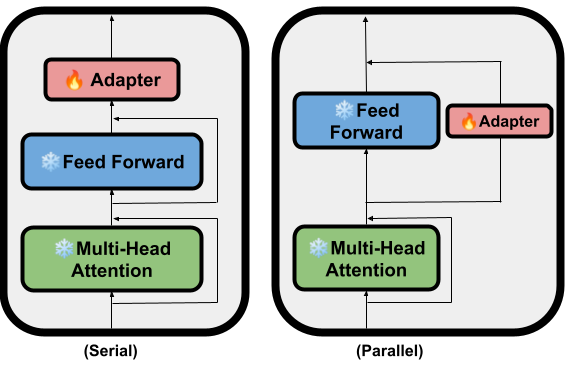
\includegraphics[scale=0.27]{imgs/Adapter_Transformer.png}
    \caption{Transformer block with various residual adapter configurations. Normalisation layers are not display in this figure}
    \label{fig:transformer_config}
    \end{center}
\end{figure*}
\begin{figure*}[t]
    \begin{center}
    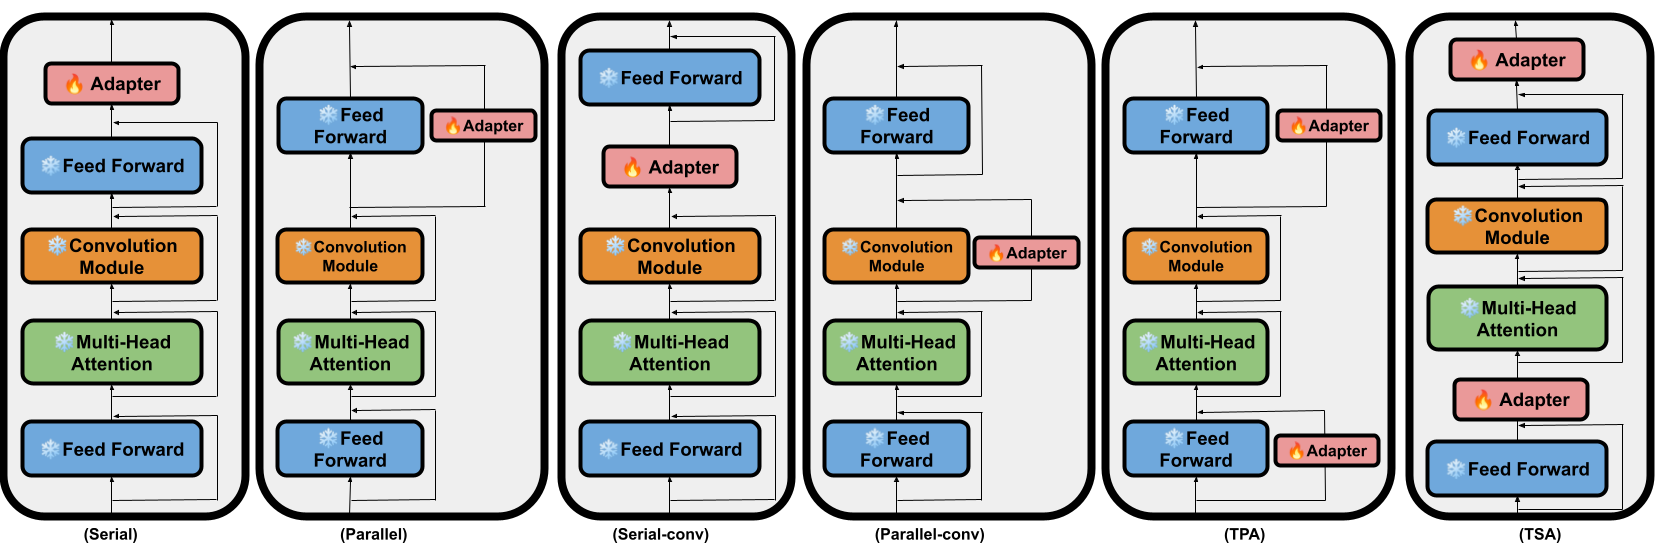
\includegraphics[scale=0.27]{imgs/Adapter_conformer.png}
    \caption{Conformer block with various residual adapter configurations. Normalisation layers are not display in this figure}
    \label{fig:conformer_config}
    \end{center}
\end{figure*}

In this section, we delve into the application of Adapter-transfer as PETL for both Transformer and Conformer architectures in the domain of children's ASR. Building upon our findings from the previous chapter, where we identified the FFN modules as the most relevant component to fine-tuning in a Transformer-based model, we opt to leverage Adapters for modifying the output of these FFN modules. Additionally, considering our results that underscore the significance of fine-tuning the Encoder, our primary emphasis will be on investigating the implementation of Adapters within the Encoder. Specifically, for the Transformer architecture, we investigate two integration methods: parallel and serial placement with the FFN component. Such configurations were used in prior work \cite{he2021towards} and are depicted in Figure \ref{fig:transformer_config}.

In the case of the Conformer architecture, we explore six distinct Adapter configurations, as illustrated in Figure \ref{fig:conformer_config}. The initial two configurations mirror our Transformer investigation, involving both parallel and serial placements, either after or in parallel with the second FFN layer \cite{chen2023efficient}. Additionally, we assess a configuration that introduces an Adapter following the convolution module, denoted as the "serial-conv" setup used in \cite{10095837}. Notably, although the FFN component has been identified as the most crucial for fine-tuning, promising results have also been observed by fine-tuning the convolution modules \cite{chen2023efficient}. Furthermore, \cite{chen2023efficient} introduces two variants of the parallel setup: "parallel-conv," where the Adapter operates in parallel with the convolution module, and "TPA," which deploys two adapters in parallel with both FFN modules in the Conformer layer. This comprehensive exploration of Adapter configurations within both architectures aims to discern the most effective adaptation strategies for children's speech in the context of ASR. 


In the case of serial configurations, the integration of adapter information is performed with the preceding component denoted as $P$. The specific component $P$ varies depending on the configuration and can be either FFN or convolution modules. This integration is realised through the following process:

\begin{equation}
    output =  Adapter(P(x))
\end{equation}

where $x$ represents the input of component $P$.

For parallel configurations, the integration process varies slightly. In this scenario, the adapter's output is combined with the output of component $P$ as follows:

\begin{equation}
    output = x + 0.5 \cdot P(x) + (Adapter(x) - x)
\end{equation}

where $x$ is the input of component $P$.

To comprehensively explore all feasible configurations, we introduce two novel setups. The first one is referred to as "Two Serial Adapters" or "TSA," where two Adapters are sequentially positioned after each FFN component in all layers. The second configuration combines TPA and TSA, resulting in the integration of four Adapter modules both in parallel and serially at the two FFN modules level. 
%To fully explore all feasible configurations, we introduce two novel configurations respectively called Two Serial Adapters or "TSA" where two Adapters are positioned sequentially after each FFN component in all layers. The second configuration is the combination of the TPA and TSA where four Adapters modules are integrated both in parallel and serial at the two FFN modules level.

Moreover, we consider three distinct configurations where Adapters are placed in the Decoder. It is important to note that in the Conformer architecture, the decoder is a regular Transformer. Therefore, we evaluate the "Serial" and "Parallel" setups. Subsequently, we investigate the combination of the most effective encoder Adapter configuration with both Decoder configurations. To the best of our knowledge, there is no prior research that formally investigates the influence of Adapters within an ASR decoder. 
%In the case of serial configurations, we integrate the adapter information with the preceding component denoted as $P$. The specific component $P$ varies depending on the configuration and can be either the FFN or the convolution modules. This integration is accomplished through the following process:
%\begin{equation}
%    output =  Adapter(P(x))
%\end{equation}
%In the parallel configurations, the integration process differs slightly. Here, we combine the adapter's output with the output of component $P$ as follows:
%\begin{equation}
%    output = x + 0.5 * P(x) + (Adapter(x) - x)
%\end{equation}
%where $x$ is the input of the component $P$. In order to comprehensively explore all feasible configurations, we introduce a novel one called ``TSA,'' which stands for Two Serial Adapters. In this configuration, one Adapter is positioned sequentially after each FFN component.

%Additionally, for a comprehensive assessment of Adapter behaviour, we consider three distinct configurations where Adapters are placed in the Decoder. Note that in the Conformer architecture, the decoder is a regular Transformer. Therefore, we initially evaluate the ``Serial''and ``Parallel''setups. Subsequently, we investigate the combination of the most effective encoder Adapter configuration with both Decoder configurations. To the best of our knowledge, there is no prior research that formally investigates the influence of Adapters within an ASR decoder.%

% Finally, we explore the use of unsupervised clustering of utterances, motivated by the strong correlation between children's speech variability and age. Our aim is to create clusters of utterances that exhibit similar acoustic characteristics. This process employs a k-means clustering algorithm on the x-vector representation \cite{snyder2018x} of each training utterance. The primary objective is to investigate whether Adapters trained on comparable speech characteristics yield improvements over a general Adapter on the entire training set. To evaluate this approach, we use this clustering in the test set, where test utterances are decoded with their respective cluster Adapters.

Finally, motivated by the observed strong correlation between children's speech variability and age, we explore the possibility of training specialised Adapters. However, considering the high inter-speaker variabilities in children's speech, using age directly may not effectively capture children with similar acoustic characteristics. Additionally, in many children's speech datasets, precise age information is often not provided. To address this, we partition the training dataset into groups of speakers with similar acoustic characteristics based on unsupervised clustering.
In practice, we apply a k-means clustering algorithm on the x-vector representation \cite{snyder2018x} of all training utterances. Subsequently, distinct Adapters are trained for each speaker cluster separately. During the testing phase, the closest clusters of group of speaker is determined for each test utterance, and the corresponding Adapters specific to that group are employed for decoding.

%Finally, motivated by the strong correlation between children's speech variability and age, we investigate the possibility of training specialized Adapters for groups of speakers exhibiting similar acoustic characteristics based on unsupervised clustering. In practice, we apply a k-means clustering algorithm on the x-vector representation \cite{snyder2018x} of each training utterance. Then, a different adapter model is trained for each  speaker cluster. During test, the closest speaker cluster is found for each test utterance and the corresponding Adapter weights are used for decoding.
The primary objective of these experiments is to investigate whether Adapters trained on comparable speech characteristics yield improvements over a general Adapter on the entire training set. Indeed,
%\subsection{Relation to prior work}
%\label{sec:prior}
% No work fully compared Adapter vs Conformer in Children speech
children's speech is inherently atypical and displays a significant degree of variability, making it imperative to assess the efficacy of existing methods. In prior work, different configurations were employed resulting in a lack of standardised evaluation.

\section{Implementation details}

All experiments were performed using the SpeechBrain toolkit \cite{speechbrain}. We used  12 Transformer or Conformer layers for the encoder, for the Transformer and Conformer model respectively, and 6 Transformer layers for the decoder, all with dimensions 512. These models have been pre-trained using the LibriSpeech dataset \cite{librispeech} and are publicly available\footnote{https://huggingface.co/speechbrain/asr-transformer-transformerlm-librispeech} \footnote{https://huggingface.co/speechbrain/asr-conformer-transformerlm-librispeech}. Furthermore, for all of our experiments, we used the same Transformer language model, trained on 10 million words 
%CAMERA-READY (Add Information about the Language model training)
on the LibriSpeech transcriptions.
The adapter architecture consists of a  first linear layer projection to dimension 512 with a ReLu activation, followed by another linear layer projection to dimension 512 with a residual connection of the adapter input. For all Adapters, in the initialisation process, we set $W_{down}$ to all zeros, and $W_{up}$, $b_{down}$, $b_{up}$ are initialised using Xavier initialisation \cite{glorot2010understanding}.


The use of a hidden-dimension size equal to the model size (instead of a bottleneck) was motivated by previous research exploring hidden-dimension size, that consistently demonstrated that larger dimensions tend to yield improved performance scores \cite{chen2023efficient}.
All models were trained for 30 epochs, with a learning rate of $8\cdot10^{-4}$ for Adapters experiments and of $8\cdot10^{-5}$ for fine-tuning the entire model.
For the clustering experiments, we use the k-means clustering algorithm on the speaker-embedding of each utterance. The speaker embeddings were extracted using a publicly pre-trained ECAPA-TDNN model, trained on adult speech\footnote{https://huggingface.co/speechbrain/spkrec-ecapa-voxceleb}.

\section{Results}
\label{sec:results}

\subsection{Configurations}
\begin{table}[t]
\caption{Results of the different Adapters configurations in both Transformer and Conformer.}
\begin{center}    
\begin{tabular}{ccc}
\hline
 Method & WER     & Trained params    \\ \hline \hline
\multicolumn{3}{c}{Transformer} \\ \hline
\multicolumn{1}{l}{\textit{Frozen}} & 25.04\%   & - \\
\multicolumn{1}{l}{\textit{Full fine-tuning}} & 12.99\% & 71.5M \\ \hline
\multicolumn{1}{l}{Serial}  &   12.78\% & 6.3M  \\ 
\multicolumn{1}{l}{Parallel}  &     \textbf{12.62\%} & 6.3M  \\ \hline\hline
\multicolumn{3}{c}{Conformer} \\ \hline
\multicolumn{1}{l}{\textit{Frozen}} & 21.75\%   & - \\ 
\multicolumn{1}{l}{\textit{Full fine-tuning}} & 12.28\% & 109.1M \\ \hline
\multicolumn{1}{l}{Serial}  &   11.76\% & 6.3M  \\ %11.84 
\multicolumn{1}{l}{Serial-Conv} & 11.78\%     & 6.3M  \\
\multicolumn{1}{l}{Parallel}    & 11.72\% & 6.3M  \\ % 11.88 
\multicolumn{1}{l}{Parallel-conv} & 11.79\%      & 6.3M  \\ %\hline
\multicolumn{1}{l}{TPA} & \textbf{11.58\%}     & 12.6M  \\ %11.85
\multicolumn{1}{l}{TSA} & 11.75\%     & 12.6M  \\ \hline %11.72
\multicolumn{1}{l}{Serial (Decoder)} & 18.09\%     & 3.2M  \\ 
\multicolumn{1}{l}{Parallel (Decoder)} &17.76\%     & 3.2M  \\ \hline
%\multicolumn{1}{l}{TPA + Serial (Decoder)} & 00.00(T)\%     & 15.8M  \\
%\multicolumn{1}{l}{TPA + Serial (Decoder)} & 11.68\%     & 15.8M  \\ 
\multicolumn{1}{l}{TPA + Parallel (Decoder)} & \textbf{11.47\%}     & 15.8M  \\ \hline

\end{tabular}
\end{center}

\label{tab:res}
\end{table}

In this section, we present a comprehensive evaluation of Adapter configurations applied to both Transformer and Conformer models, assessing their performance based on Word Error Rate (WER), as presented in Table \ref{tab:res}.  First, we assess 
%CAMERA-READY ( remove this to make more clear that frozen is no-finetune and without adapters)
%Adapter configurations in 
the Transformer model when no fine-tuning was applied (\textit{Frozen}), resulting in a WER of 25.04\%. Conversely, \textit{Full Fine-Tuning} involved complete fine-tuning of the entire model,
%CAMERA-READY (Make more clear that this is our baseline)
working as our baseline system
, reducing the WER significantly to 12.99\%, at the expense of 71.5 million trainable parameters.
Turning to the Adapter setups, we investigate the ``Serial'' and ``Parallel'' configurations, both equipped with 6.3 million trainable parameters. The ``Parallel''emerged as the best configuration, achieving the lowest WER of 12.62\% compared to 12.78\% for the ``Serial``. These results underscore the effectiveness of Adapter configurations within the Transformer architecture, as they both perform slightly better than the full-finetuning.

Next, we investigated the Conformer model, we once again explored \textit{Frozen} and \textit{Full Fine-Tuning}. In \textit{Frozen} the pre-trained model remained untouched, yielding a WER of 21.75\%. The Full fine-tuning, in a similar way as the Transformer, led to enhanced performance, reducing the WER to 12.28\% with a total of 109.1 million trainable parameters. We can observe that given the same pre-training dataset, the Conformer architecture outperforms the regular Transformers. Within the set of adapter configurations, ``Serial'' achieved a WER of 11.76\%, while ``Parallel'' demonstrated slightly better performance with a WER of 11.72\%. These results indicated that ``Parallel''Adapters were more effective in improving WER in the Conformer model. When Adapters are placed after the convolution layer, with the ``Serial-conv'' and ``Parallel-conv'' configuration, both slightly under-perform compared to Adapters placed after the second FFN component with respective scores of 11.78\% and 11.79\%. Finally, we evaluated the ``TPA''and ``TSA''configurations. The ``TPA''configuration emerged as the most promising, with a very remarkable WER of 11.58\% using 12.6 million trainable parameters, while ``TSA''achieved a WER of 11.75\%, which is slightly under-performing compared to the ``TPA''configuration.

In addition, we evaluated the use of  Adapters in the decoder. As the decoder of the Conformer architecture is a regular Transformer, we only evaluate the ``Serial''and ``Parallel'' setup, which respectively reached 18.09\%  and 17.76\% WER with 3.2 million parameters. Results showed that Adapters are more relevant when plugged into the encoder. It confirms that acoustic variability plays a critical role in the degradation of children's ASR performance. Finally, combining ``TPA''in the encoder layers with ``Parallel''Adapters in the decoder outperforms Adapters in the encoder only, with 11.47\% WER. Consequently, this configuration stands as the most effective model. 

%statistical tests
We performed statistical tests (Matched Pairs Sentence-Segment Word Error) across all Adapter setups in comparison to the full fine-tuning configuration using SCTK, the NIST Scoring Toolkit \footnote{https://github.com/usnistgov/SCTK/tree/master}. 
The results reveal that, in all scenarios, the \textit{p}-value is less than or equal to 0.001. This observation denotes statistical significance, indicating evidence against the null hypothesis. 

These results collectively illustrate the versatility and effectiveness of different Adapter configurations within the Transformer and  Conformer model for the children's ASR task. ``TPA''Adapters in the Encoder combined with ``Parallel''Adapters in the Decoder showcased outstanding performance, highlighting their potential as a fine-tuning replacement in large model children ASR scenarios.

\subsection{Unsupervised Clustering of utterances}
\begin{table}[t]
\caption{Results of the clustering approach.}
\begin{center}    
\begin{tabular}{cc}
\hline
  \# of clusters & Average WER     \\ \hline
\multicolumn{1}{c}{1} & 11.58\%  \\% OR 11.70%  If we consider 40 epochs instead of 30 here
\multicolumn{1}{c}{2} & \textbf{11.50\%}  \\
\multicolumn{1}{c}{3} & 11.57\%  \\
\multicolumn{1}{c}{4} & 11.51\%  \\ \hline 

\end{tabular}
\end{center}

\label{tab:res_clusters}
\end{table}



In this section, we present the outcomes of our clustering approach, as summarised in Table \ref{tab:res_clusters}. We investigated the influence of varying cluster numbers on ASR performance, ranging from 1 to 4 clusters using the ``TPA''in the encoder-only configuration. Notably, when the data remained unclustered (one cluster), the ASR system exhibited a WER of 11.58\%. However, the two-cluster configuration surpassed the others, achieving a superior performance of 11.50\%. This result suggests that partitioning the data into two distinct clusters enables the Adapters to more effectively capture underlying patterns intricately linked to their respective clusters, consequently enhancing the recognition scores. Furthermore, we explored the impact of increasing the number of clusters to three and four, revealing only marginal differences in performance, with WERs of 11.57\% and 11.51\%, respectively. These findings underscore the role of data clustering in children's ASR systems.

\section{Exploring PETL alternative approaches}
As PETL gains more and more attention from the research community, an array of novel architectures and methodologies has emerged, extending beyond the conventional Adapters. These innovative approaches have been extensively explored in various domains such as NLP and image processing but remain relatively unexplored in the domains of speech processing and, notably, children's ASR.

The objective of this section is to analyze these emerging PETL methods specifically in the context of children's ASR. Drawing from our prior findings, which underscored the significance of fine-tuning FFN modules, we have curated a selection of PETL approaches designed to be integrated with FFN. Notably, we excluded PETL approaches centered around the MHSA modules, such as LORA, as well as any prompt-related PETL strategies like prompt tuning.

This section starts with a in-depth presentation of the selected PETL. Each chosen methodology is thoroughly described, elucidating its underlying principles, architectural intricacies, and key characteristics conpared to the traditional Adapter. 
Following, we assess the performances of these selected PETL methodologies  in the specific context of children's ASR. The evaluation encompasses various dimensions, including performances compared to the full-finetuning and parameter-efficiency. By systematically benchmarking these alternative PETL methodologies against the conventional Adapter models, our objective is to not only understand the individual strengths and limitations of these approaches but also to evaluate their relative effectiveness in tackling the specific challenges presented by children's ASR.


\subsection{Scaled Adapters}
% Explain the idea has been used in many example
Scaled or Gated Adapters extend the conventional residual Adapters by introducing a scaling mechanism to the output of the Adapter modules. The concept of scaled-Adapters was initially introduced by \cite{he2022towards} and is formally expressed as:
\begin{equation}
    adapter(x) = x + s \cdot (W_{up}(f(W_{down}g(x) + b_{down})) + b_{up})    
\end{equation}
% Tunable parameters
Here, $s \in \mathbb{R}$ is a tunable scalar hyperparameter. Notably, some research has proposed the to learn directly this scalar value during training as a gate mechanism \cite{mao-etal-2022-unipelt}. The intuition behind this approach is to allow the network to gradually learn to assign weights to the target domain, achieving more fine-grained control of the Adapter activation or deactivation. The scaled learning process facilitates the regulation of contributions from the Adapters from differents layers, enabling the model to adapt and refine its responses based on the specific characteristics of the data encountered during training.
% Experimental setup
Within the context of our experiments, we decided to use a trainable scalar associated to each Adapter modules. This scaling parameters and all Adapter modules were optimised through a 30 epochs training using a learning rate of $8 \times 10^{-4}$.

\subsection{Convolution based Adapters}
% CNN make sense for speech
Convolutional Neural Networks have been widely recognised for their effectiveness in exploiting local information, particularly for computer vision tasks. These networks learn shared kernels based on position within localised windows, giving them the ability to capture features such as edges and shapes. This characteristic has also been demonstrated in the field of speech-related tasks, as demonstrated by the success of the Conformer architecture \cite{gulati2020conformer}.

%Then CNN in Adapter is a normal step
As a result of this success, CNNs have been naturaly incorporated into Adapter modules. This strategic fusion enables Adapters to leverage the spatial processing capabilities inherent in convolutional modules, thereby enhancing their capacity to capture and adapt to different patterns present in the data. The initial approach involved using CNNs as feature extractors, in conjunction with a linear transformation, as detailed by \cite{yang23p_interspeech}, we denoted this approach as Conv-Adapter. We experimented two version of Conv-Adapters, where a 1-dimensional CNN is used as replacement of either the first of second linear of the traditional Adapters. More formally, the \textit{$\text{Conv-Adapter}_{down}$} expressed as followed:
\begin{equation}
    \text{Conv-adapter}_{Down}(x) = x + (W_{up}(\text{CNN}_{1D}(x))+ b_{up})
\end{equation}
While \textit{$\text{Conv-Adapter}_{up}$} is defined as:
\begin{equation}
    \text{Conv-adapter}_{up}(x) = x + \text{CNN}_{1D}(W_{down}(x)+ b_{down})
\end{equation}
We also investigated, the \cite{muthuchamyselvaraj23_interspeech} Conv-Adapter where the CNN is integrated in between the Up and Down projection of the traditional Adapter, denoted \textit{$\text{Conv-Adapter}_{Middle}$}, mathematically expressed as:
\begin{equation}
    \text{Conv-adapter}_{Middle}(x) = x + W_{up}(\text{CNN}_{1D}(W_{down}(x)+ b_{down})+ b_{up})
\end{equation}

\begin{figure}
    \begin{center}
        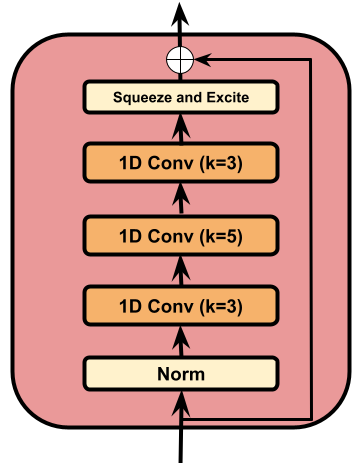
\includegraphics[scale=0.4]{imgs/ConvPass.png}
        \caption{Th architecture of the ConvPass adapter. $k$ is the kernel size of the 1D convolution. All Convoluation are depth-wise convolution.}
        \label{fig:convpass}
    \end{center}
\end{figure}

% Adapter fully CNN based
An alternative approach involves the use of a fully CNN-based Adapter known as ConvPass, which has demonstrated effectiveness in computer vision tasks \cite{jie2022convolutional}. Diverging from conventional Adapters and the previously mentioned Conv-Adapter, ConvPass distinguishes itself by the removal of the up and down linear layers, replaced instead by three CNN layers. In \cite{jie2022convolutional}, these layers comprise a $1 \times 1$ convolution, followed by a $3 \times 3$ convolution, and another $1 \times 1$ convolution. Notably, GELU activation functions are interposed between these convolutional layers.

For speech-related tasks, a comparable approach was introduced by \cite{li2023evaluating}. The speech-specific ConvPass, illustrated in Figure \ref{fig:convpass}, incorporates a layer normalisation layer, followed by three lightweight 1-dimensional CNN layers with kernel sizes of 3, 5, and 3, respectively. Additionally, a squeeze and excite module is integrated into the architecture. The squeeze and excite module, as proposed by \cite{hu2018squeeze}, facilitates feature recalibration. It consists of a global pooling operation, followed by a linear layer, a Rectified Linear Unit (ReLU) activation, a second linear layer, and concludes with a Sigmoid activation.

During our experiments, all Conv-Adapters and ConvPass configurations were trained for 30 epochs with a learning rate of $8 \times 10^{-4}$.
%Alternatively is possibe to use a fully CNN-based Adapter. Called ConvPass, it was found effective for computer vision tasks \cite{jie2022convolutional}. ConvPass differ from regular Adapter and previously mentioned Conv-Adapter as the up and down linear layers were removed and replaced with three CNN layers, a $1 \times 1$ followed by a $3 \times 3$ and finally a $1 \times 1$ with GELU activation in between them. In speech, a similar approach was proposed by  \cite{li2023evaluating}. The speech ConvPass, presented in figure \ref{fig:convpass}, consist of layer normalisation layer, followed by 3 lightweight 1-dimensional CNN with kernel size of 3, 5 and 3 respectively along with a squeeze and excite module. Squeeze and excite module \cite{hu2018squeeze} allows a feature recalibration and is consisted of a global pooling, one linear layer, a Relu activation and second linear layer followed by a Sigmoid.

\subsection{BitFit}
Bias-Term Fine-Tuning, known as BitFit, is a PETL method introduced by \cite{ben-zaken-etal-2022-bitfit} for NLP tasks. The main idea behind BitFit is to fine-tune only the bias terms and the task-specific classification layer while keeping the rest of the model frozen. This approach aims to achieve efficient fine-tuning with reduced computational requirements in a similar way as our partial fine-tuning experiments in chapter \ref{chap:e2e}. The fine-tuning of bias terms can be seen as introducing a task-specific shift to the token representations.

%Advantages of Bitfit
The authors highlight three key properties of BitFit. Firstly, it matches of a fully fine-tuned model, showcasing its ability to maintain comparable results while significantly reducing the number of parameters to be trained. Secondly, BitFit is designed to adapt to tasks arriving sequentially, eliminating the need for simultaneous access to all datasets. This adaptability enhances the model's versatility in handling diverse tasks with varying data distributions over time. Thirdly, BitFit exhibits parameter efficiency by fine-tuning only a small subset of the model's parameters.

%Experimental setup
In our experiment, the pre-trained model and children's ASR task shared the same output dimensions and character encoding. In consequence, we excluded the fine-tuning of the task-specific classification layer. The training process consisted of 30 epochs with a learning rate of $8 \times 10^{-4}$.

\subsection{Scale and Shift features}
% Define SSF
Scale and Shift features (SSF) was introduced an PETL alternative approach by Lian and al. \cite{lian2022scaling} for image classification. The primary objective of SSF is to establish a generalised method for efficient model fine-tuning without the introduction of task-specific inference parameters. Drawing inspiration from feature modulation techniques such as \cite{wu2018group,huang2017arbitrary}, the SSF method modulate deep features extracted by a pre-trained model by scaling and shifting them to match the distribution of a target dataset. 
The intuition behind SSF comes from the inherent disparities in data distributions between upstream and downstream datasets. Directly applying model weights trained on an upstream dataset to a downstream dataset frequently leads to a performance degradation due to the disparities between the two datasets \cite{sun2016return}. The SSF method addresses this challenge by introducing scale $\gamma$ and shift $\beta$ parameters, which could be considered as the variance and mean used to modulate the features extracted from the pre-trained model. This modulation ensures that the adapted features align with the characteristics of the upstream dataset. Formally, given an input $x$, the modulated output $y$ is calculated by:
\begin{align}
    y = \gamma \odot x + \beta
\end{align}

Notably, the scale and shift parameters in SSF remain independent on any input and have a unified learnable parameter-space for different tasks. Another noteworthy advantage of SSF is its reliance on linear transformations, which can be seamlessly merged into the original pre-trained weights during model re-parameterization in the inference phase. This integration avoid the need for additional parameters removing the extra-computation time of other PETL such as Adapters.

% How to put it in a model
In practical terms, SSF are introduced after each modules within the Conformer architecutre (FFNs, MHSA and Convolution modules). In the original paper, they also finetuned the Head-layers as the task is a image classification task, as our both upstream and downstream tasks, respectively adult and children ASR, share the same output dimension and character encoding, we do not finetune this extra layer and only use the SSF method. 

%Experimental setup
In practice, the SSF modulation is integrated after each operations of the neural network. For our experiments, each operations corespond the different modules within the Conformer architecture, specifically the FFNs, MHSA and Convolution modules. It is noteworthy that, in the original paper, the authors also fine-tuned an Head-layer, as the output of the upstream and downstream image classification tasks are different. However, in our experiment, both the upstream and downstream tasks involve English ASR with shared output dimensions and characters encoding. Therefore,we did not include the head-layer fine-tuning and exclusively employed the SSF method. Our training compromise 30 epochs with a learning rate of $8\cdot10^{-4}$.


\subsection{AdapterBias}
\begin{figure}
    \begin{center}
        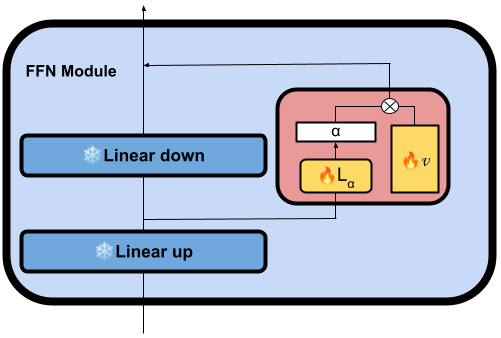
\includegraphics[scale=0.4]{imgs/AdapterBias.png}
        \caption{ AdapterBias, consisting of a linear layer $L_\alpha$ and a vector $\mathcal{V}$, is added after the second feed-forward layer only in each FFN module.}
        \label{fig:AdapterBias}
    \end{center}
\end{figure}
% Link to Bitfit
Following the success of BitFit \cite{ben-zaken-etal-2022-bitfit}, which aims to introduce task-specific shifts to each output representation by selectively fine-tuning only the bias terms of a pre-trained model, recent research has suggested that certain tokens may hold more significance than others for specific tasks. While BitFit uniformly applies the same shift across all tokens regardless of their relevance to the task, \cite{fu-etal-2022-adapterbias} proposes AdapterBias to address this limitation.

% What is AdapterBias
AdapterBias comprises two essential modules: a vector $\mathcal{V}$ and a linear layer $L_\alpha$. The vector $\mathcal{V}$ represents a task-specific shift added to the output of each FFN modules, acknowledging that tokens more closely related to the task should be assigned to larger representation shifts than others. On the other hand, the linear layer $L_\alpha$ generates a token-dependent weight vector $\alpha = [\alpha_1, \alpha_2, ..., \alpha_m]^T$, where $\alpha_i$ is the weight associated with the representation shift of the $i^{th}$ token. By applying these token-specific weights to the task-specific representation shift $\mathcal{V}$, AdapterBias focuses on tokens which are more crucial to the task, allowing efficient and fine adaptation to various downstream tasks.

The output of AdapterBias is defined as the bias (B), represented as the outer product of $\mathcal{V}$ and the learned weights vector $\alpha$. Mathematically, the output of AdapterBias is expressed as follows:

\begin{equation}
    B = \mathcal{V} \otimes \alpha^T    
\end{equation}

Here, \(\otimes\) denotes the element-wise multiplication of the task-specific shift vector \(\mathcal{V}\) and the token-dependent weight vector \(\alpha\).
% Experimental seting
In our experimental setup, we conducted the training for AdapterBias by integrating them into the second linear layer of each of the two FFN modules within the Conformer architecture. We trained AdapterBias for 30 epochs, employing a learning rate of $8 \times 10^{-4}$.

\section{Results of the different PETL methods}

\begin{figure}
    \begin{center}
        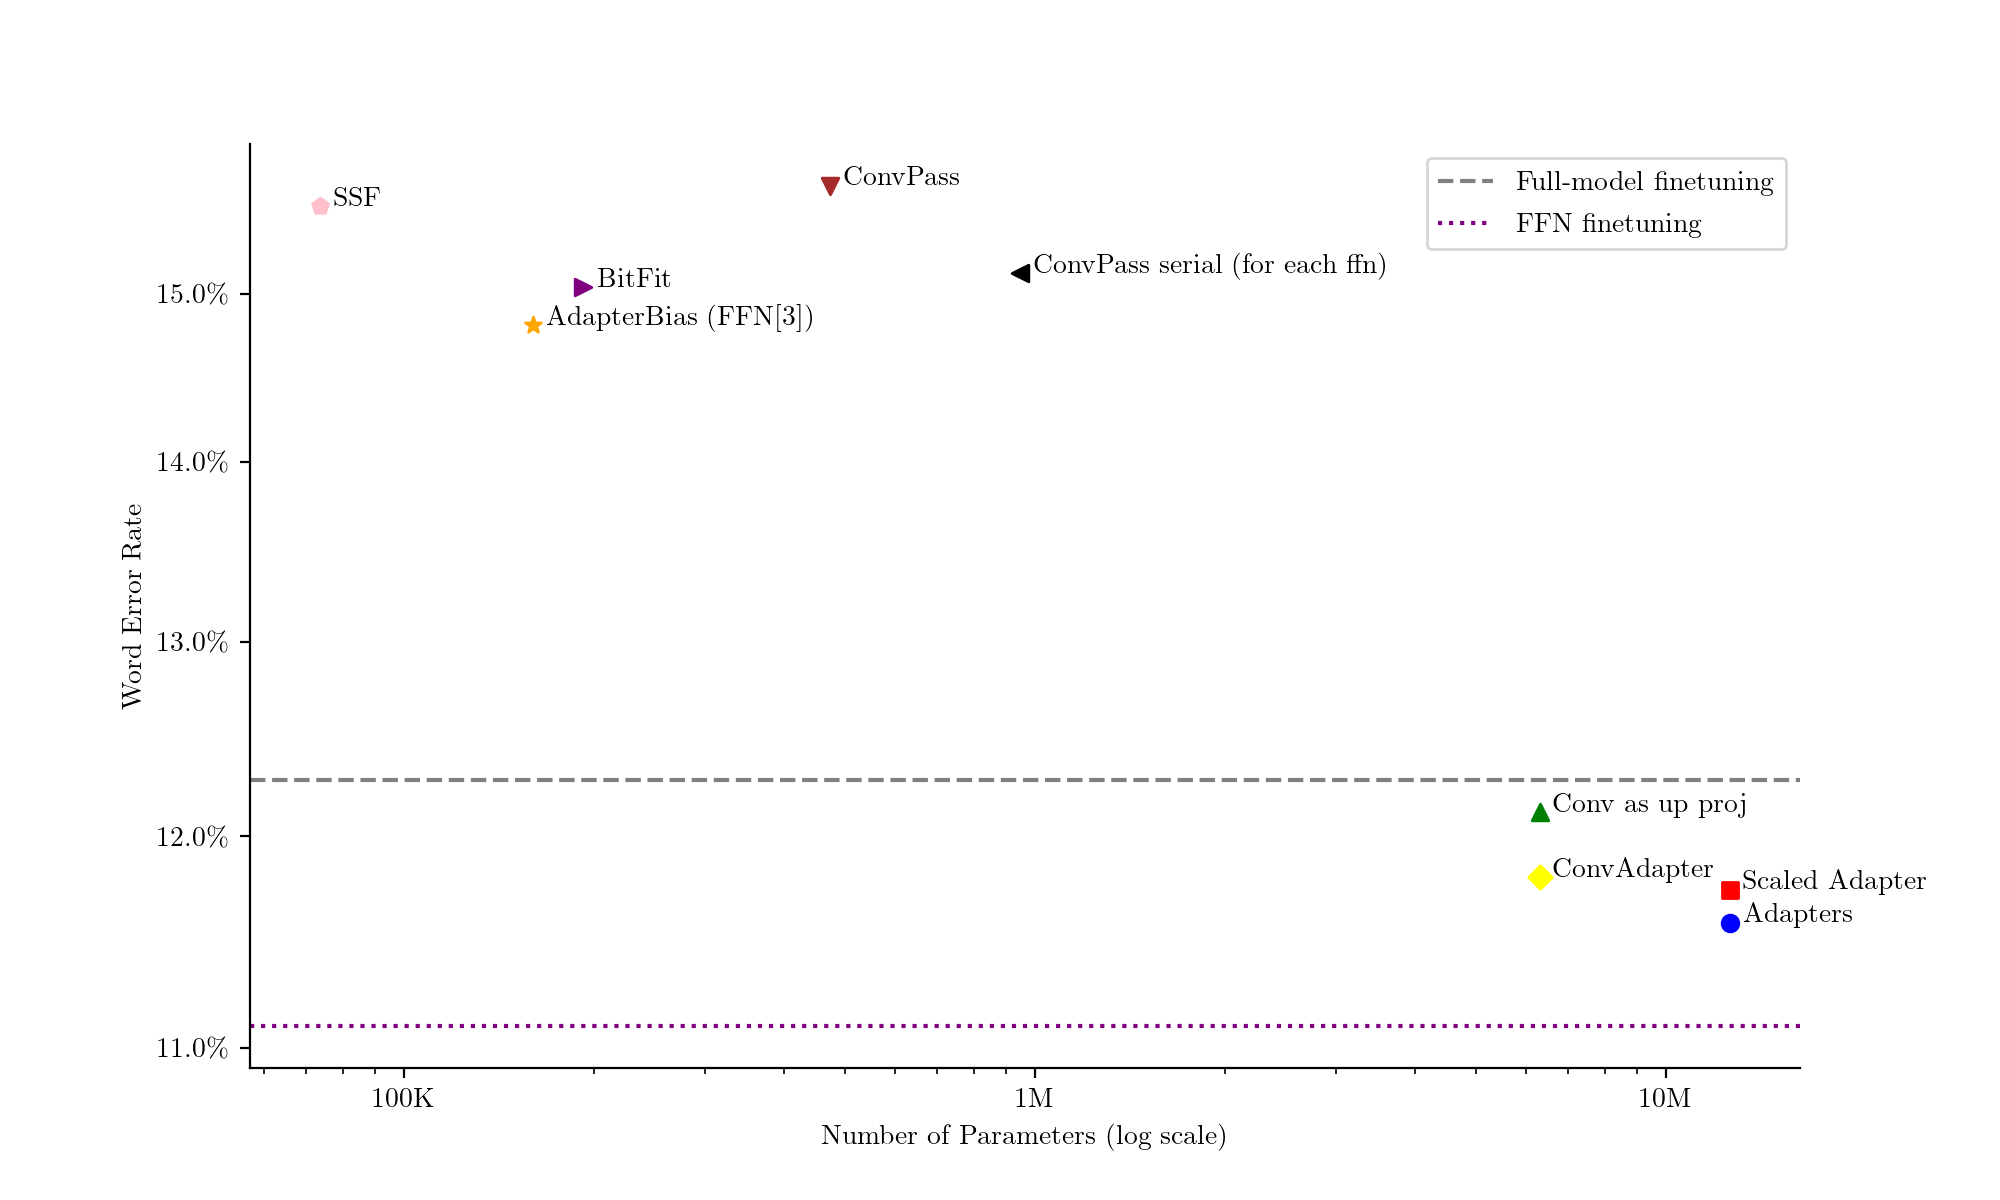
\includegraphics[width=\textwidth]{imgs/Adapter_compare_withoutWide.png}
        \caption{Different paramter efficent procedure for children ASR in conformer model}
        \label{fig:adapter_compared_withoutWide}
    \end{center}
\end{figure}




\section{Shared Adapter}
% Goal PETL- Good score, small |param|
The primary objective of PETL is to either maintain or surpass the performance achieved through full fine-tuning of a pre-trained model, while minimising the number of parameters employed. In previous sections, the efficiency of residual Adapters has been underscored. Remarkably, using only 10\% of the total number of parameters compared to the fine-tuning of the entire model, these residual Adapters exhibit superior performances in the context of children's ASR. In addition, with our experiments we highlighted the drawback and presence of overparameterisation in Transformer-based models.

% FFN redundancy
Leveraging this understanding, we propose a novel PETL methodology developed on the concept of sharing residual Adapters. The inspiration for this approach draws from the insights provided by the work of \cite{pires2023one}, which focus on the FFN modules. Despite representing a significant proportion of the model's parameters, the FFN was identified as highly redundant. This affirmation is confirmed by the work of \cite{geva2020transformer}, which  establishes a connection between the FFN and attention mechanisms by proposing that the FFN corresponds to learnable key-value pairs. In this conceptualisation, the weights of the first layer of the FFN represent the keys, while those of the second layer correspond to the values. These keys are proficient at capturing salient patterns at each layer. Interestingly, they observed that the classes of patterns tend to overlap between neighboring layers, indicating redundancy in the representation. This observation underscores the potential for optimising PETL methods by addressing and mitigating redundancy within the FFN, ultimately contributing to more parameter-efficient transfer learning processes.

% Shared FFN work
Building upon this insightful observation, \cite{pires2023one} modified the conventional Transformer architecture by sharing and dropping the FFN across different layers. Their investigation confirms the substantial degree of redundancy between the FFNs of the encoder and decoder components. Consequently, they successfully eliminate the decoder FFN while sharing a single FFN across the encoder, achieving a noteworthy reduction in model parameters without significant compromise to accuracy.

Formally, denoting the number of encoder layers as $N_{enc}$, the sharing of the FFN modules in the encoder can be expressed as follows:

\begin{equation}
    \text{FFN}_{i}^{enc}(.) = \text{FFN}^{enc}_{all}(.) , \forall i: 1 \leq i \leq N_{enc}
\end{equation}

%Shared Adapter motivation
In light of the success observed with the shared FFN in the encoder, we hypothesise that the presence of redundancy within the FFN might lead to a similar redundancy issue when employing one Adapter per FFN layer. In other words, employing separate Adapters for different layers might also exhibit redundancy. To address this concern, we introduced the Shared Adapter approach, wherein a singular Adapter is used across all layers. This approach aims to alleviate redundancy in the context of multiple FFN layers while reducing the total amount of parameters used in Adapter-transfer. The formal expression of the Shared Adapter is presented as follows:

\begin{equation}
    \text{Adapter}_{i}(.) = \text{Adapter}_{all}(.) , \forall i: 1 \leq i \leq N_{enc}
\end{equation}

% Experimental seting for shared Adapters

\begin{figure}
    \begin{center}
        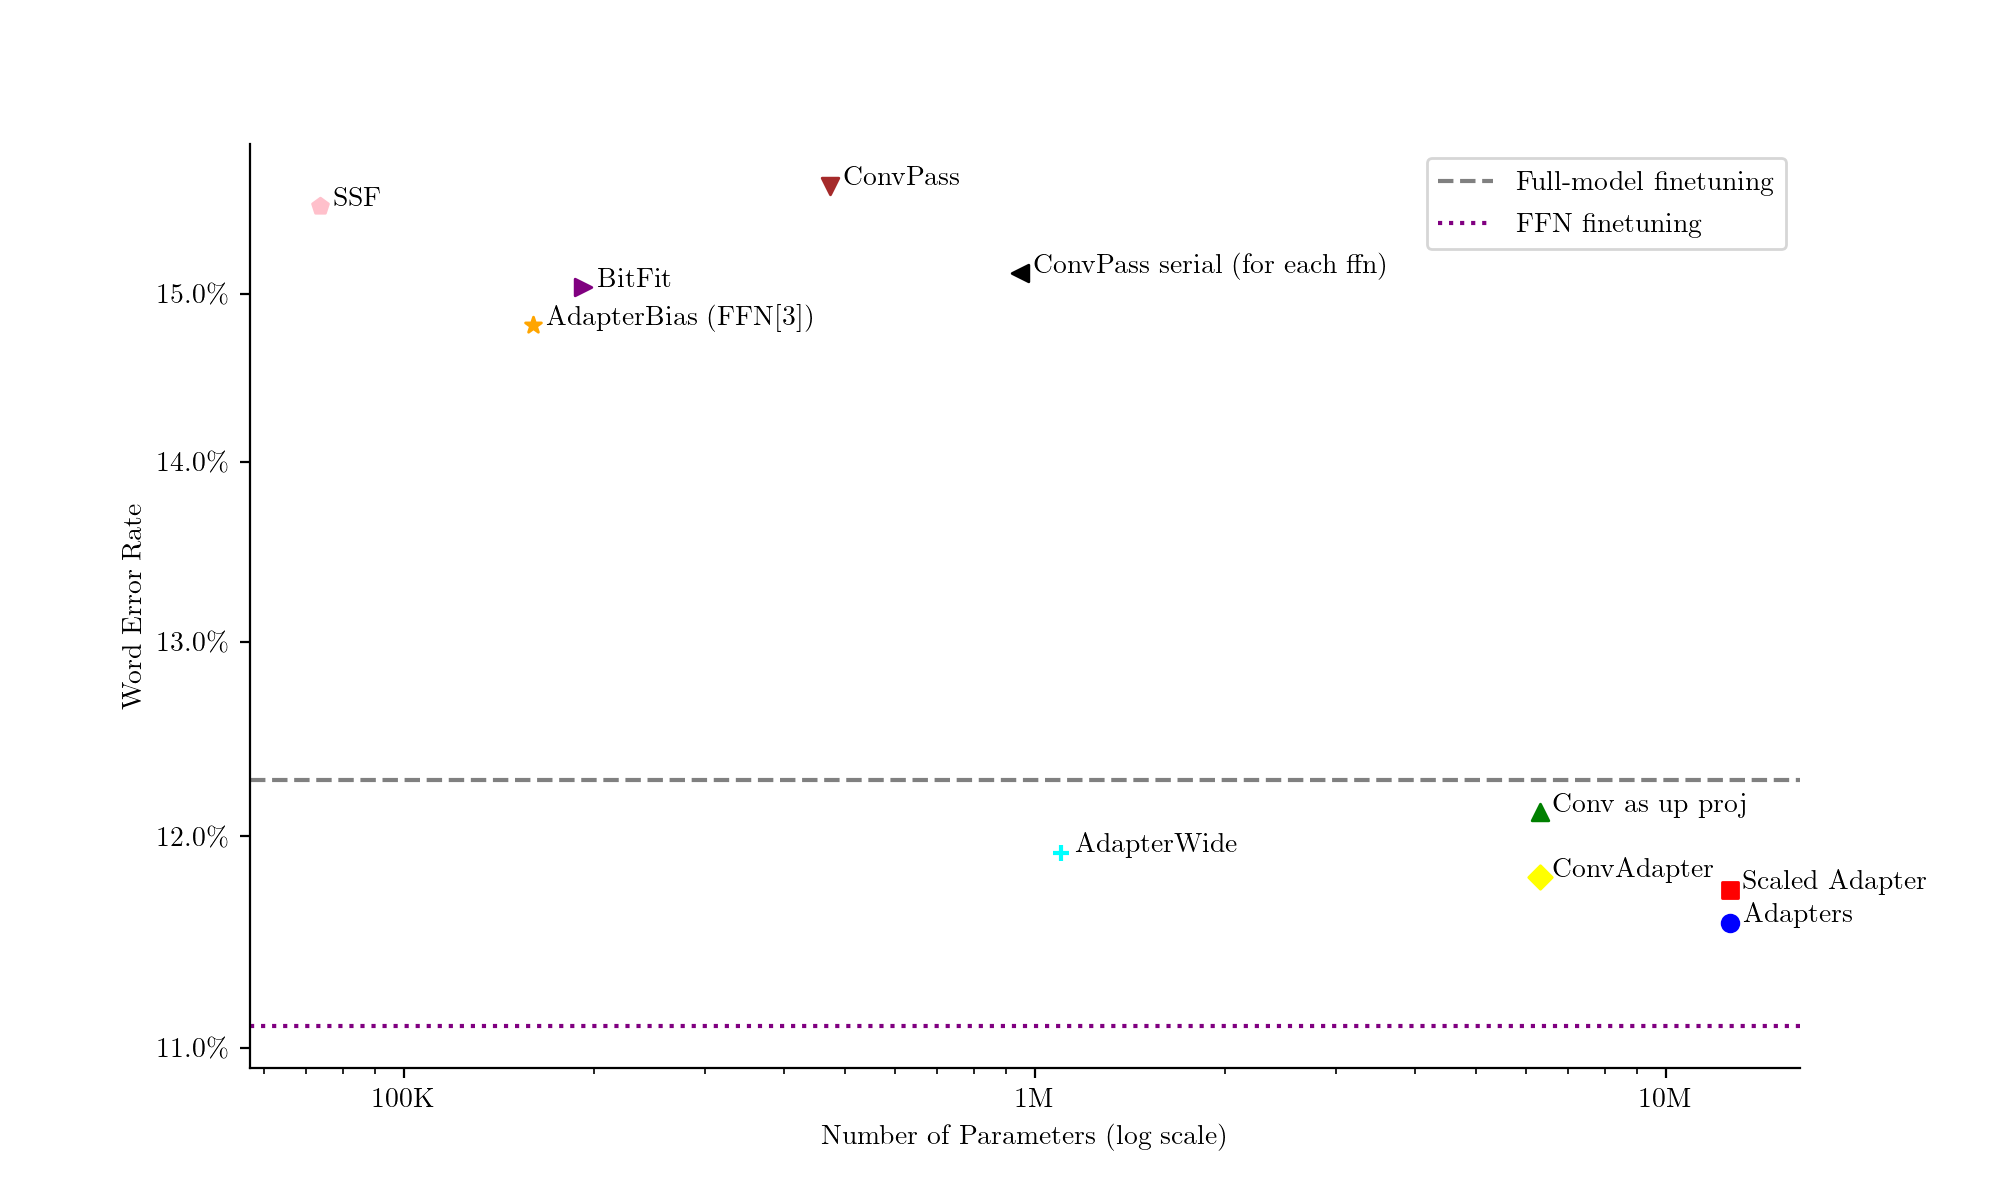
\includegraphics[width=\textwidth]{imgs/Adapters_compare.png}
        \caption{Different paramter efficent procedure for children ASR in conformer model with shared-Adapters}
        \label{fig:adapter_compared}
    \end{center}
\end{figure}
\begin{figure}
    \begin{center}
        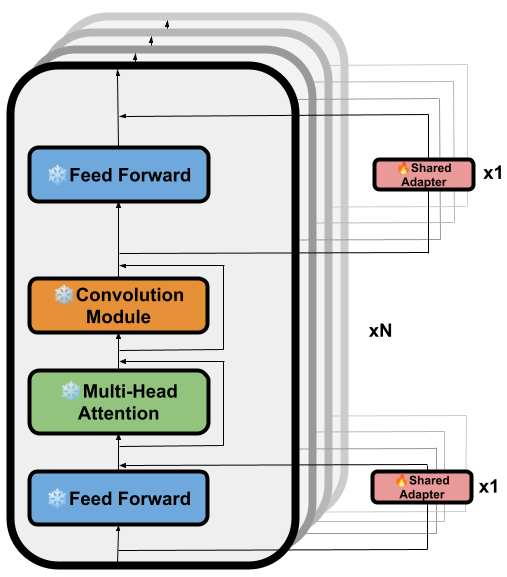
\includegraphics[scale=0.3]{imgs/Shared_Adapters.png}
        \caption{Shared-Adapter setup in a Conformer model}
        \label{fig:Shared_adapter}
    \end{center}
\end{figure}


%  SSL

The final research direction we want to explore in this thesis is self-supervised learning (SSL) as a front-end feature rather than typical filter banks or MFCCs. For these models, the training process is separated into two stages. The first phase of training is self-supervised, which implies that no labels are used during training. The objective of this first phase is to present a large amount of unlabelled data to the system so that it learns a good speech representation. The second stage of learning is supervised fine-tuning, in which the model is taught to predict specific phonemes using the robust representation acquired in the previous stage with the help of a small amount of labelled data. In this category, two models stand out as state-of-the-art: Wav2Vec 2.0 \cite{baevski2020wav2vec} and HuBert \cite{hsu2021hubert}. As a preliminary experiment, to asses the usability of such frameworks for children ASR, we trained a BiLSTM model using the output of a variety of frozen self-supervised systems. For this experiment we used a subset of 50h of the Myst corpus \cite{MyST}, and the preliminary findings are displayed in the table \ref{tab:ssl}
\begin{table}[ht]
\centering
\begin{tabular}{lcc} 
\hline
Front-end & UER & WER \\ 
\hline
Fbanks & 12.29\% & 35.14\% \\ 
\hline
TERA \cite{tera} & 11.31\% & 31.80\% \\
Audio Albert \cite{chi2021audio} & 12.28\% & 34.69\% \\
Wav2Vec2.0 Base & 7.37\% & 19.76\% \\
Wav2Vec2.0 Large~ & 7.00\% & 18.76\% \\
Distill HuBert \cite{chang2022distilhubert} & 9.22\% & 25.75\% \\
HuBert Base & 7.40\% & 19.77\% \\
HuBert Large & \textbf{6.03\%} & \textbf{15.41\%} \\
\hline
\end{tabular}
\caption{Results without language model of Self-supervised front-end}
\label{tab:ssl}
\end{table}

Where Base, and Large represent the same model with different number of parameters (in the order Base $<$ Large).
Even though we did not use a language model in this pilot experiment, the results are of the same order as those reported in section \ref{section:exp} obtained with a transformer and a transformer language model. Such results demonstrate that SSL learns substantial speech characteristics. For future research, we aim to explore in depth what information is encoded in SSL models and why they work well on children, and how we may use this knowledge to enhance children's ASR.
